% Chapter 9

\chapter{The second wire, the Fermi Hamiltonian} % Main chapter title

\label{Chapter9} % For referencing the chapter elsewhere, use \ref{Chapter9} 

\lhead{Chapter 9. \emph{The 2nd wire, Fermi Hamiltonian}} % This is for the header on each page - perhaps a shortened title

%----------------------------------------------------------------------------------------
In the chapter we will study the fermion Hamiltonian. Firstly, we will make the mean field approximation analogous to the one in chapter \ref{Chapter4}. Secondly, we will use this to write up the gap equations for the resulting pairing potentials. Finally, we will write up the total grand Hamiltonian for the fermions. 

\section{The interaction Hamiltonian and the mean field approximation}
The interaction Hamiltonians for the intrawire interactions of the fermions are the same as the one studied in chapter \ref{Chapter4}. This also means, that we get analogous gap equations for the pairing potentials internally in wire 1 and 2 (see equation \ref{eq.pairingpotentialdef}) :
\begin{align}
\Delta^{11}_k &= -\frac{1}{\mathcal{L}} \sum_k W^\text{ind}_{FF,11}(k,k')\braket{f_{1,k'}f_{1,-k'}}, \nonumber \\
\Delta^{22}_k &= -\frac{1}{\mathcal{L}} \sum_k W^\text{ind}_{FF,22}(k,k')\braket{f_{2,k'}f_{2,-k'}}, \nonumber \\
W^\text{ind}_{FF,11}(k,k') &= W^\text{ind}_{FF,22}(k,k') = \frac{1}{2}\left[V^\text{ind}_{FF}(k-k',0) - V^\text{ind}_{FF}(k+k',0) \right].
\label{eq.pairingpotentialsintrawire}
\end{align}

However, this does not mean, that $\Delta^{11}_k = \Delta^{22}_k$, since $\braket{f_{1,k'}f_{1,-k'}}$ and $\braket{f_{2,k'}f_{2,-k'}}$ can potentially be different. We will return to this later on. The above pairing potentials are associated with the following terms of the total $H^\text{int}_{FF}$:
\begin{align}
H^\text{int}_{FF,11} &= \frac{1}{2}\sum_k \left[\Delta^{11}_k f^\dagger_{1,k}f^\dagger_{1,-k} - \Delta^{11 *}_k f_{1,k}f_{1,-k} - \Delta^{11}_k\braket{f^\dagger_{1,k}f^\dagger_{1,-k}} \right], \nonumber \\
H^\text{int}_{FF,22} &= \frac{1}{2}\sum_k \left[\Delta^{22}_k f^\dagger_{2,k}f^\dagger_{2,-k} - \Delta^{11 *}_k f_{2,k}f_{2,-k} - \Delta^{22}_k\braket{f^\dagger_{2,k}f^\dagger_{2,-k}} \right].
\label{eq.Hintintrawire}
\end{align}

The interaction Hamiltonian for the interwire interactions is:
\begin{equation}
H^\text{int}_{FF,12} = \int dx dx' \psi^\dagger_{1,F}(x)\psi^\dagger_{2,F}(x') \tilde{V}^\text{ind}_{FF}(x-x',0) \psi_{2,F}(x')\psi_{1,F}(x).
\end{equation}
The factor in front of $1/2$ is absent, since the fermions in wire 1 and 2 are distinguishable. The mean field in this situation is $\braket{\psi_{2,F}(x')\psi_{1,F}(x)}$. Performing the mean field approximation analogously to the calculation in chapter \ref{Chapter4} then shows, that:
\begin{equation}
H^\text{int}_{FF,12} = \frac{1}{\mathcal{L}} \sum_{k,k'} V^\text{ind}_{FF,12}(k-k',0)\left[\braket{f_{2,k'}f_{1,-k'}}f^\dagger_{1,-k}f^\dagger_{2,k} + \braket{f^\dagger_{1,-k'}f^\dagger_{2,k'}}f_{2,k}f_{1,-k} - \braket{f_{2,k'}f_{1,-k'}}\braket{f^\dagger_{1,-k}f^\dagger_{2,k}} \right].
\end{equation}

We therefore define the interwire pairing potential as:
\begin{equation}
\Delta^{12}_k = -\frac{1}{\mathcal{L}} \sum_{k'} V^\text{ind}_{FF,12}(k-k',0)\braket{f_{2,k'}f_{1,-k'}}.
\end{equation}

This brings the interaction part of the interwire Hamiltonian on the following form:\footnote{As for the single wire, this is technically no longer an interaction Hamiltonian, since it is only quadratic in the operators.}
\begin{equation}
H^\text{int}_{FF,12} = \sum_{k} \left[\Delta^{12}_k f^\dagger_{2,k}f^\dagger_{1,-k} + \Delta^{12 *}_k f_{1,-k}f_{2,k} - \Delta^{12}_k\braket{f^\dagger_{2,k}f^\dagger_{1,-k}} \right].
\label{eq.Hintinterwire}
\end{equation}
Equations \ref{eq.Hintintrawire} and \ref{eq.Hintinterwire} are the essential equations for the following. 

\section{The grand fermion Hamiltonian}
The grand fermion Hamiltonian is obtained in a similar manner to the single wire analog. The free fermion part is now: $H_{0,1}+H_{0,2} = \sum_{j,k}\frac{k^2}{2m_F}f^\dagger_{j,k}f_{j,k}$. Further, the Hamiltonian is not particle number conserving, since it contains terms like $f^\dagger f^\dagger$. In stead we impose diffusive equilibrium by subtracting $\mu_1N_{1,F}+\mu_2N_{2,F}$. $\mu_j$ is the chemical potential of wire $j$ and $N_{j,F} = \sum_k f^\dagger_{j,k}f_{j,k}$ is the number of $j$ fermions. We hereby get the following grand Hamiltonian:
\begin{align}
H_{FF} &= \sum_j \left[H_{0,j} - \mu_j N_{j,F}\right] + H^\text{int}_{FF,11} + H^\text{int}_{FF,22} + H^\text{int}_{FF,12} \nonumber \\
       &= \frac{1}{2}\sum_k\left[\varepsilon_{1,k} + \varepsilon_{2,k} - \Delta^{11}_k\braket{f^\dagger_{1,k}f^\dagger_{1,-k}} - \Delta^{22}_k\braket{f^\dagger_{2,k}f^\dagger_{2,-k}} - 2\Delta^{12}_k\braket{f^\dagger_{2,k}f^\dagger_{1,-k}} \right] + \frac{1}{2}\sum_k F^\dagger_k \mathcal{H}_{FF,k}F_k,
\end{align}

with:
\begin{equation}
\mathcal{H}_{FF,k} = \begin{bmatrix} \varepsilon_{1,k} & \Delta^{11}_k      & 0                 & -\Delta^{12}_{-k} \\ 
                                     \Delta^{11 *}_k   & -\varepsilon_{1,k} & \Delta^{12*}_k    & 0 \\ 
                                    0                  & \Delta^{12}_k      & \varepsilon_{2,k} & \Delta^{22}_k \\ 
                                     -\Delta^{12*}_{-k}& 0                  & \Delta^{22*}_k    & -\varepsilon_{2,k} \end{bmatrix}, \hspace{0.5cm}
F_k =  \begin{bmatrix} f_{1,k} \\ f^\dagger_{1,-k} \\ f_{2,k} \\ f^\dagger_{2,-k} \end{bmatrix}.                                     
\end{equation}
Here $\varepsilon_{j,k} = \frac{k^2}{2m_F}-\mu_j$ is the kinetic energy relative to the chemical potential of the $j$ fermions. This has a quite general structure. To simplify matters we firstly assume, that the wires are held at the same chemical potential $\mu$. Hence we let $\varepsilon_{j,k} \to \varepsilon_k$. Secondly, we wish to investigate, whether we can find real solutions for the intrawire pairings $\Delta^{jj}_k$. First of all, since the two wires are equivalent, the pairing potentials have to equal up to a phase: $\Delta^{11}_k = \text{e}^{i\phi_k} \Delta^{22}_k$. Second, we can gauge transform the phase of $\Delta^{jj}_k$ away in the same way as in chapter \ref{Chapter7}. Since this gauge transformation can be done independently for each wire, we obtain $\Delta^{11}_k = \Delta^{22}_k$. The interwire pairing $\Delta^{12}_k$ describes a pairing between distinguishable particles. If we think of the wires as indexed with a pseudospin, the pairing is expected to be a $s$-wave type pairing. We will therefore search for an even solution for $\Delta^{12}_k$. This means, that:
\begin{equation}
\mathcal{H}_{FF,k} = \begin{bmatrix} \varepsilon_{k}   & \Delta^{11}_k      & 0                 & -\Delta^{12}_{k} \\ 
                                     \Delta^{11}_k     & -\varepsilon_{k}   & \Delta^{12*}_k    & 0 \\ 
                                    0                  & \Delta^{12}_k      & \varepsilon_{k}   & \Delta^{11}_k \\ 
                                     -\Delta^{12*}_{k} & 0                  & \Delta^{11}_k     & -\varepsilon_{k} \end{bmatrix},                  
\end{equation}
As for the single wire the eigenvalues of the kernel above come in plus/minus pairs. The norm of the eigenvalues give the energy dispersion. The result is:
\begin{equation}
E^{\pm}_{F,k} = \sqrt{\varepsilon^2_k + \left(\Delta^{11}_k\right)^2 + \left(\Delta^{12}_k\right)^2 \pm \left|2\Delta^{11}_k\text{Im}\left[\Delta^{12}_k\right]\right|}, 
\end{equation} 
Analogous to the single wire this will lead to an energy decrease of the ground state, which increases with $E^{+}_{F,k} + E^{-}_{F,k}$. See equation \eqref{eq.Kitaev.HFF_diagonal} for the single wire case. From the form of the energy dispersion we see, that this energy decrease is largest, when the pairing is real. To see this explicitly we first define: $E_{F,k} = \sqrt{\varepsilon^2_k + \left(\Delta^{11}_k\right)^2 + \left(\Delta^{12}_k\right)^2}$. We then see, that we have to maximize the function:
\begin{equation}
E^{+}_{F,k} + E^{-}_{F,k} = \sqrt{E^2_{F,k} + \left|2\Delta^{11}_k\text{Im}\left[\Delta^{12}_k\right]\right|} + \sqrt{E^2_{F,k} - \left|2\Delta^{11}_k\text{Im}\left[\Delta^{12}_k\right]\right|}. \nonumber
\end{equation}
This is equivalent to finding the maximum of the function $f(x) = \sqrt{1 + x} + \sqrt{1 - x}$, which is obtained for $x = 0$. This explicitly shows, that the phase of the interwire pairing is not arbitrary, when the phases of the intrawire pairings have been chosen. The restriction of least ground state energy ensures, that there is only a single energy dispersion:
\begin{equation}
E_{F,k} = \sqrt{\varepsilon^2_k + \left(\Delta^{11}_k\right)^2 + \left(\Delta^{12}_k\right)^2}.
\label{eq.energydispersiontwowires}
\end{equation}
Finally, the new quasiparticle operators are found by finding the eigenvectors to $\mathcal{H}_{FF,k}$. We define the quasiparticle fermionic operators $\zeta_{j,k}$ by:
\begin{equation}
\begin{bmatrix} f_{1,k} \\ f^\dagger_{1,-k} \\ f_{2,k} \\ f^\dagger_{2,-k} \end{bmatrix} = U_{F,k}\begin{bmatrix} \zeta_{1,k} \\ \zeta^{\dagger}_{1,-k} \\ \zeta_{2,k} \\ \zeta^{\dagger}_{2,-k} \end{bmatrix}.
\label{eq.zetaoperatorstwowiresdefinition}
\end{equation} 
The $\zeta$ operators have to obey the same anticommutation relations as the $f$ operators. Specifically anticommutators like $\{\zeta_1, \zeta_2 \} $ vanishes. $\mathcal{H}_{FF,k}$ should then be diagonalised to yield:
\begin{equation}
U^\dagger_{FF,k}\mathcal{H}_{FF,k}U_{FF,k} = \begin{bmatrix} 
E_{F,k} & 0        & 0       & 0        \\ 
0       & -E_{F,k} & 0       & 0        \\ 
0       & 0        & E_{F,k} & 0        \\ 
0       & 0        & 0       & -E_{F,k} \\ 
\end{bmatrix} \nonumber
\end{equation}
Further the diagonalisation must respect the symmetry in the 1 and 2 fermions of the Hamiltonian. Specifically the assumption of $\Delta^{22}_k = \Delta^{11}_k$ must be selfconsistent. From \ref{eq.pairingpotentialsintrawire} this means, that $\braket{f_{1,k}f_{1,-k}} = \braket{f_{2,k}f_{2,-k}}$. This results in the following matrix:
\begin{equation}
U_{F,k} = \frac{1}{(2E_{F,k}(E_{F,k}+\varepsilon_k))^{1/2}}\begin{bmatrix} 
E_{F,k}+\varepsilon_k & \Delta^{11}_k             & 0                      & -\Delta^{12}_k           \\  
\Delta^{11}_k         & -(E_{F,k}+\varepsilon_k)  & \Delta^{12}_k          & 0                        \\ 
0                     & \Delta^{12}_k             & E_{F,k}+\varepsilon_k  & \Delta^{11}_k           \\ 
-\Delta^{12}_k        & 0                         & \Delta^{11}_k          & -(E_{F,k}+\varepsilon_k)
\end{bmatrix}. \nonumber
\end{equation}
Notice, that the structure of $U_{F,k}$ and $\mathcal{H}_{FF,k}$ is very similar. The diagonalisation of the Hamiltonian is now straight forward. $U^\dagger_{F,k}\mathcal{H}_{FF,k}U_{F,k}$ is diagonal with the eigenvalues $+E_{F,k}$ and $-E_{F,k}$ alternating in the diagonal as shown above. The result of the diagonalisation is therefore:
\begin{align}
H_{FF} &= E_0 + \sum_{j,k} E_{F,k}\zeta^\dagger_{j, k}\zeta_{j, k}, \nonumber \\ 
E_0 &= \sum_k \left[\varepsilon_k - E_{F,k} - \frac{1}{2}\left(\Delta^{11}_k\braket{f^\dagger_{1,k}f^\dagger_{1,-k}} + \Delta^{22}_k\braket{f^\dagger_{2,k}f^\dagger_{2,-k}} + 2\Delta^{12}_k\braket{f^\dagger_{2,k}f^\dagger_{1,-k}} \right) \right] 
\end{align}  
We notice, that indeed the ground state energy $E_0$ is lowered by $E_{F,k}$ as previously argued. This confirms, that we have chosen the correct phase of the interwire pairing $\Delta^{12}_k$. As for the single wire case the ground state is hereby defined by $\zeta_{j,k}\ket{\text{S}}_0 = 0$. 

\section{The gap and number equations}
In this section we write up and discuss the gap equations. They are derived in complete analogy to the single wire case. By combining $U_{F,k}$ and equation \ref{eq.zetaoperatorstwowiresdefinition} we can transform to the quasiparticle operators $\zeta$. Further, the quasiparticles obey Fermi statistics: $\braket{\zeta^\dagger_{j,k}\zeta_{j, k}} = f(E_{F,k})$, where $f$ is the Fermi-Dirac distribution. The gap equations hereby become:
\begin{align}
\Delta^{11}_k = \Delta^{22}_k &= -\frac{1}{\mathcal{L}}\sum_{k'} W^\text{ind}_{FF,11}(k,k')\frac{\Delta^{11}_{k'}}{2E_{F,k'}}\tanh\left(\frac{\beta E_{F,k'}}{2}\right), \nonumber \\
\Delta^{12}_k &= -\frac{1}{\mathcal{L}}\sum_{k'} V^\text{ind}_{FF,12}(k - k',0)\frac{\Delta^{12}_{k'}}{2E_{F,k'}}\tanh\left(\frac{\beta E_{F,k'}}{2}\right).
\end{align}
This explicitly shows, that the assumption of the intrawire pairings, $\Delta^{22}_k = \Delta^{11}_k$, is self-consistent. The assumption of $\Delta^{12}_k$ being even in $k$ is also seen to be self-consistent. Further, we notice that the gap equations have the exact same structure as the ones for the single wire. Finally, these gap equations goes to the gap equations for the separated single wires found in chapter \ref{Chapter4} when $\Delta^{12}_k$ goes to $0$.  

It turns out that the number equation calculated from $N_F = \sum_k \braket{f^\dagger_{j,k}f_{j,k}}$ has the exact same structure as the single wire number equation as well. Explicitly: 
\begin{equation}
n_F = \int \frac{dk}{2\pi} \frac{\varepsilon_k}{E_{F,k}}f(E_{F,k}) + \frac{1}{2}\left(1 - \frac{\varepsilon_k}{E_{F,k}}\right). 
\label{eq.numberequationtwowires}
\end{equation}
This gives us three integral equations for the three quantities: $\Delta^{11}_k, \Delta^{12}_k$ and $\mu(T)$.

\begin{figure} 
\begin{center}  
% GNUPLOT: LaTeX picture with Postscript
\begingroup
  \makeatletter
  \providecommand\color[2][]{%
    \GenericError{(gnuplot) \space\space\space\@spaces}{%
      Package color not loaded in conjunction with
      terminal option `colourtext'%
    }{See the gnuplot documentation for explanation.%
    }{Either use 'blacktext' in gnuplot or load the package
      color.sty in LaTeX.}%
    \renewcommand\color[2][]{}%
  }%
  \providecommand\includegraphics[2][]{%
    \GenericError{(gnuplot) \space\space\space\@spaces}{%
      Package graphicx or graphics not loaded%
    }{See the gnuplot documentation for explanation.%
    }{The gnuplot epslatex terminal needs graphicx.sty or graphics.sty.}%
    \renewcommand\includegraphics[2][]{}%
  }%
  \providecommand\rotatebox[2]{#2}%
  \@ifundefined{ifGPcolor}{%
    \newif\ifGPcolor
    \GPcolorfalse
  }{}%
  \@ifundefined{ifGPblacktext}{%
    \newif\ifGPblacktext
    \GPblacktexttrue
  }{}%
  % define a \g@addto@macro without @ in the name:
  \let\gplgaddtomacro\g@addto@macro
  % define empty templates for all commands taking text:
  \gdef\gplbacktext{}%
  \gdef\gplfronttext{}%
  \makeatother
  \ifGPblacktext
    % no textcolor at all
    \def\colorrgb#1{}%
    \def\colorgray#1{}%
  \else
    % gray or color?
    \ifGPcolor
      \def\colorrgb#1{\color[rgb]{#1}}%
      \def\colorgray#1{\color[gray]{#1}}%
      \expandafter\def\csname LTw\endcsname{\color{white}}%
      \expandafter\def\csname LTb\endcsname{\color{black}}%
      \expandafter\def\csname LTa\endcsname{\color{black}}%
      \expandafter\def\csname LT0\endcsname{\color[rgb]{1,0,0}}%
      \expandafter\def\csname LT1\endcsname{\color[rgb]{0,1,0}}%
      \expandafter\def\csname LT2\endcsname{\color[rgb]{0,0,1}}%
      \expandafter\def\csname LT3\endcsname{\color[rgb]{1,0,1}}%
      \expandafter\def\csname LT4\endcsname{\color[rgb]{0,1,1}}%
      \expandafter\def\csname LT5\endcsname{\color[rgb]{1,1,0}}%
      \expandafter\def\csname LT6\endcsname{\color[rgb]{0,0,0}}%
      \expandafter\def\csname LT7\endcsname{\color[rgb]{1,0.3,0}}%
      \expandafter\def\csname LT8\endcsname{\color[rgb]{0.5,0.5,0.5}}%
    \else
      % gray
      \def\colorrgb#1{\color{black}}%
      \def\colorgray#1{\color[gray]{#1}}%
      \expandafter\def\csname LTw\endcsname{\color{white}}%
      \expandafter\def\csname LTb\endcsname{\color{black}}%
      \expandafter\def\csname LTa\endcsname{\color{black}}%
      \expandafter\def\csname LT0\endcsname{\color{black}}%
      \expandafter\def\csname LT1\endcsname{\color{black}}%
      \expandafter\def\csname LT2\endcsname{\color{black}}%
      \expandafter\def\csname LT3\endcsname{\color{black}}%
      \expandafter\def\csname LT4\endcsname{\color{black}}%
      \expandafter\def\csname LT5\endcsname{\color{black}}%
      \expandafter\def\csname LT6\endcsname{\color{black}}%
      \expandafter\def\csname LT7\endcsname{\color{black}}%
      \expandafter\def\csname LT8\endcsname{\color{black}}%
    \fi
  \fi
    \setlength{\unitlength}{0.0500bp}%
    \ifx\gptboxheight\undefined%
      \newlength{\gptboxheight}%
      \newlength{\gptboxwidth}%
      \newsavebox{\gptboxtext}%
    \fi%
    \setlength{\fboxrule}{0.5pt}%
    \setlength{\fboxsep}{1pt}%
\begin{picture}(7200.00,5040.00)%
    \gplgaddtomacro\gplbacktext{%
      \csname LTb\endcsname%
      \put(814,767){\makebox(0,0)[r]{\strut{}$0$}}%
      \csname LTb\endcsname%
      \put(814,1469){\makebox(0,0)[r]{\strut{}$0.1$}}%
      \csname LTb\endcsname%
      \put(814,2170){\makebox(0,0)[r]{\strut{}$0.2$}}%
      \csname LTb\endcsname%
      \put(814,2872){\makebox(0,0)[r]{\strut{}$0.3$}}%
      \csname LTb\endcsname%
      \put(814,3573){\makebox(0,0)[r]{\strut{}$0.4$}}%
      \csname LTb\endcsname%
      \put(814,4275){\makebox(0,0)[r]{\strut{}$0.5$}}%
      \csname LTb\endcsname%
      \put(814,4976){\makebox(0,0)[r]{\strut{}$0.6$}}%
      \csname LTb\endcsname%
      \put(1009,484){\makebox(0,0){\strut{}$0.71$}}%
      \csname LTb\endcsname%
      \put(1828,484){\makebox(0,0){\strut{}$0.72$}}%
      \csname LTb\endcsname%
      \put(2646,484){\makebox(0,0){\strut{}$0.73$}}%
      \csname LTb\endcsname%
      \put(3465,484){\makebox(0,0){\strut{}$0.74$}}%
      \csname LTb\endcsname%
      \put(4284,484){\makebox(0,0){\strut{}$0.75$}}%
      \csname LTb\endcsname%
      \put(5103,484){\makebox(0,0){\strut{}$0.76$}}%
      \csname LTb\endcsname%
      \put(5921,484){\makebox(0,0){\strut{}$0.77$}}%
      \csname LTb\endcsname%
      \put(6740,484){\makebox(0,0){\strut{}$0.78$}}%
    }%
    \gplgaddtomacro\gplfronttext{%
      \csname LTb\endcsname%
      \put(176,2871){\rotatebox{-270}{\makebox(0,0){\strut{}$Delta_k/epsilon_{F,0}$}}}%
      \put(3874,154){\makebox(0,0){\strut{}$k_Fd$}}%
      \csname LTb\endcsname%
      \put(3385,4803){\makebox(0,0)[r]{\strut{}$Intrawire pairing$}}%
      \csname LTb\endcsname%
      \put(3385,4583){\makebox(0,0)[r]{\strut{}$Interwire pairing$}}%
    }%
    \gplbacktext
    \put(0,0){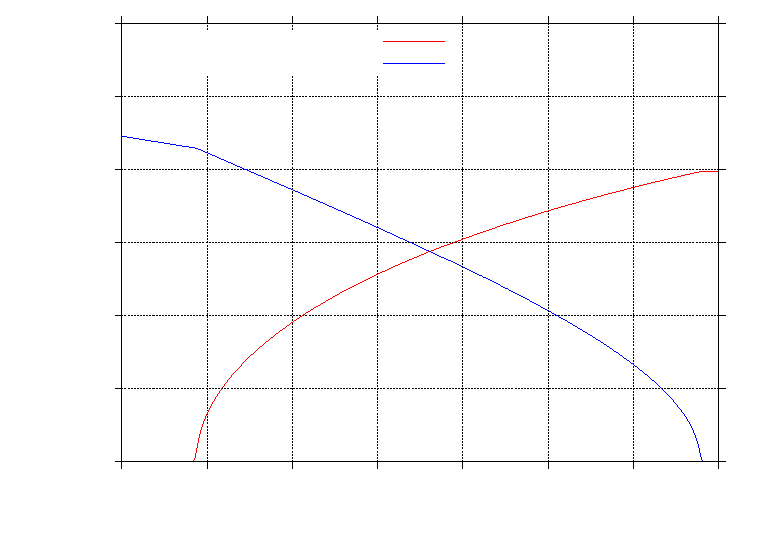
\includegraphics{ddepend}}%
    \gplfronttext
  \end{picture}%
\endgroup
  
\caption{The pairings $\Delta^{11}_k$ and $\Delta^{12}_k$ in red and blue plotted as a function of the distance $d$ between the wires. For the used set of parameters $k_F\frac{\xi}{\sqrt{2}} = 0.95$. We hereby see, that the cross over from $p$-wave dominated to $s$-wave dominated happens for $\frac{\sqrt{2}d}{\xi} \approx 0.6$. Parameters: $(n_Ba_B^3)^{1/3} = 0.01$, $(n_Ba_{BF}^3)^{1/3} = 0.1$, $l_t = 0$, $\frac{m_B}{m_F} = 7/40$, $\frac{n_F}{n_B^{1/3}} = 0.215$, $\frac{m_F^2}{m_B^2}\frac{n_B}{n_F^3} k_Fa_B = 22.10$. }  
\label{fig.maximalpairingddepend}  
\end{center}    
\end{figure}

\section{Symmetries}
In this section we will show, that the system has a time reversal symmetry that squares to unity: $T^2 = \mathbb{I}$. We will further shortly discuss the particle-hole and sublattice symmetries. 

Explicitly we define:
\begin{equation}
T\begin{bmatrix} f_{1,k} \\ f_{2,k} \end{bmatrix} T^{-1} = i\sigma_1 \begin{bmatrix} f_{1,-k} \\ f_{2,-k} \end{bmatrix} = i\begin{bmatrix} f_{2,-k} \\ f_{1,-k} \end{bmatrix},\nonumber
\end{equation} 
with $\sigma_1$ the first Pauli matrix. Hence, under this time reversal transformation a fermion from wire 1 is transformed into a fermion in wire 2 and acquires an overall phase $i$. Since $\varepsilon_{1,k} = \varepsilon_{2,k}$, the only problematic terms under time reversal are $\Delta^{11}_k f^\dagger_{1,k}f^\dagger_{1,-k}, \Delta^{22}_k f^\dagger_{2,k}f^\dagger_{2,-k}$ and $\Delta^{12}_kf^\dagger_{2,k}f^\dagger_{1,-k}$. We remember, that time reversal is antiunitary: $TiT^{-1} = -i$. This means, that the first transform according to:
\begin{equation}
\Delta^{11}_k f^\dagger_{1,k}f^\dagger_{1,-k} \overset{T}{\to} \Delta^{11*}_k \left(-i f^\dagger_{2,-k}\right)\left(-i f^\dagger_{2,k}\right) = \Delta^{11}_k f^\dagger_{2,k}f^\dagger_{2,-k}. \nonumber
\end{equation}
Here we use, that similarly to the above $Tf^\dagger_{1,k}T^{-1} = -i f^\dagger_{2,-k}$. Further, we use that $\Delta^{11}_k$ is chosen to be real. This term should be identical to the original term connected to the product $f^\dagger_{2,k}f^\dagger_{2,-k}$: $\Delta^{22}_k f^\dagger_{2,k}f^\dagger_{2,-k}$. This is exactly the case, since the intrawire pairings are chosen identical: $\Delta^{11}_k = \Delta^{22}_k$. The transformation of $\Delta^{22}_k f^\dagger_{2,k}f^\dagger_{2,-k}$ leads to the same result. Finally:
\begin{equation}
\Delta^{12}_k f^\dagger_{2,k}f^\dagger_{1,-k} \overset{T}{\to} \Delta^{12*}_k \left(-i f^\dagger_{1,-k}\right)\left(-i f^\dagger_{2,k}\right) = \Delta^{12}_k f^\dagger_{2,k}f^\dagger_{1,-k}. \nonumber
\end{equation}
This explicitly shows time reversal invariance of the above term. Further, it emphasizes that to be time reversal invariant, the interwire pairing $\Delta^{12}_k$ has to be real, when the intrawire pairings are chosen real and equal. Hence, the choice of phase that makes the system invariant under this time reversal transformation is the same choice of phase, which minimizes the ground state energy.\footnote{Had we chosen the phases of the intrawire pairings differently we could ensure a time reversal symmetry by changing the overall phase acquired under $T$.} Finally, since $i\sigma_1(-i\sigma_1) = \sigma_1^2 = \mathbb{I}$, $T$ squares to the identity.  

Similarly to the single wire case we can define a particle-hole transformation, that effectively does not change the spinor $F_k$, since the Hamiltonian of this two wire system is still of the Bogoliubov-de Gennes type. Explicitly we let:
\begin{equation}
C\begin{bmatrix} f_{j,k} \\ f^\dagger_{j,-k} \end{bmatrix}C^{-1} = \sigma_1 \begin{bmatrix} f^\dagger_{j,-k} \\ f_{j,k} \end{bmatrix} = \begin{bmatrix} f_{j,k} \\ f^\dagger_{j,-k} \end{bmatrix}, 
\end{equation} 
both for $j=1$ and $j=2$. It is then clear, that the total spinor $F_k$ is also unaffected by the transformation. As a result the Hamiltonian is invariant under $C$, and $\sigma_1^2 = \mathbb{I}$ so the transformation squares to unity. 

This analysis also gives us a sublattice symmetry: $S = TC$. In total this puts the system in Cartan class BDI with a topological index in the integers, $\mathbb{Z}$. See table \ref{tab.PeriodicTableTISC} for the details. 




